\chapter{Screenshots delle pagine Web}

\begin{figure}[h]
\centering
\includegraphics[width= 14cm]{homepage.jpg}
\caption{\textit{Homepage}}\label{homepage}
\end{figure}

\begin{figure}[h]
\centering
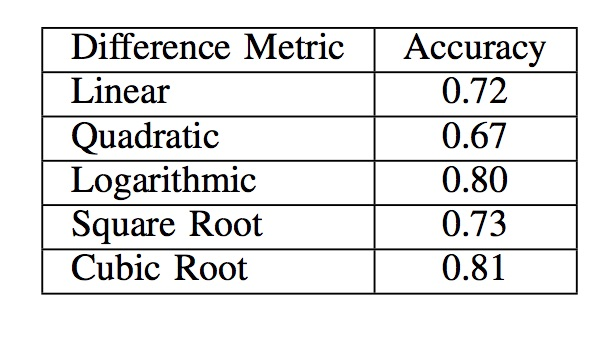
\includegraphics[width= 14cm]{results.jpg}
\caption{\textit{Risultati della ricerca}}\label{results}
\end{figure}

\begin{figure}[h]
\centering
\includegraphics[width= 14cm]{my-collection.jpg}
\caption{\textit{Collezione personale}}\label{my-collection}
\end{figure}

\begin{figure}[h]
\centering
\includegraphics[width= 14cm]{video-component.jpg}
\caption{\textit{Componente per video}}\label{video-component}
\end{figure}

\begin{figure}[h]
\centering
\includegraphics[width= 14cm]{image-component.jpg}
\caption{\textit{Componente per immagini}}\label{image-component}
\end{figure}

\begin{figure}[h]
\centering
\includegraphics[width= 14cm]{audio-component.jpg}
\caption{\textit{Componente per audio}}\label{audio-component}
\end{figure}

\begin{figure}[h]
\centering
\includegraphics[width= 14cm]{document-component.jpg}
\caption{\textit{Componente per documenti}}\label{document-component}
\end{figure}

\begin{figure}[h]
\centering
\includegraphics[width= 14cm]{upload-page.jpg}
\caption{\textit{Pagina di upload media}}\label{upload-page}
\end{figure}

\begin{figure}[h]
\centering
\includegraphics[width= 14cm]{edit-profile-page.jpg}
\caption{\textit{Pagina modifica profilo personale}}\label{edit-profile-page}
\end{figure}